\documentclass[12pt]{article}

\usepackage{times}
\usepackage{graphicx}

\setlength{\textwidth}{6.5in}
\setlength{\textheight}{8.9in}
\setlength{\oddsidemargin}{0.0in}
\setlength{\topmargin}{0.05in}
\setlength{\headheight}{-0.05in}
\setlength{\headsep}{0.0in}

\begin{document}

\begin{center}
{\bf CS 6300} \hfill {\large\bf HW05: Policy Iteration and TD Learning} \hfill {\bf Due Feb 28, 2023}
\end{center}

\noindent
Please use the \LaTeX\ template to produce your writeups. See the
Homework Assignments page on the class website for details.  Hand in
via gradescope.


\section{Temporal Difference Learning}

  \begin{center}
  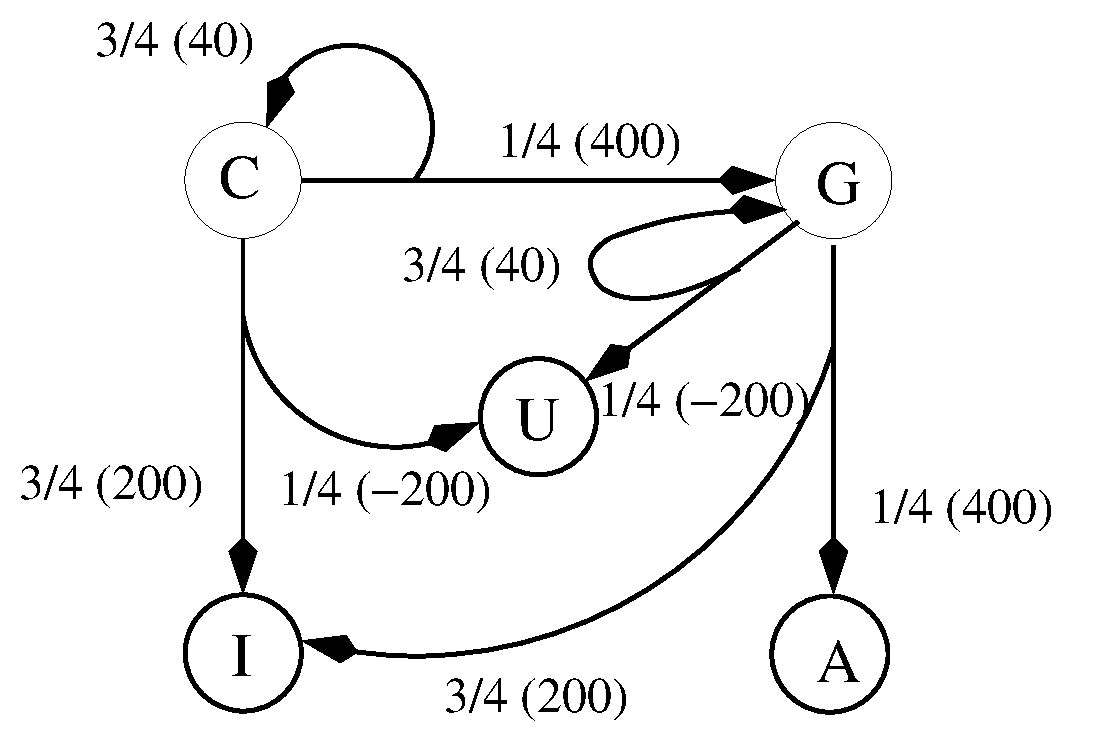
\includegraphics[height=2.5in]{cgiau.eps}
  \end{center}

For the MDP above, you decide to use experience and TD learning to
find the values.  You experience the following 3 episodes.

\begin{center}
\begin{tabular}{ccr|ccr|ccr} \hline
S & A & R    & S & A & R   & S & A & R   \\ \hline
C & s & 40   & C & s & 40  & C & s & 400 \\
C & s & 40   & C & g & 200 & G & s & 40  \\
C & s & 400  & I &   &     & G & g & 400 \\
G & s & 40   &   &   &     & A &   &     \\
G & s & -200 &   &   &     &   &   &     \\
U &   &      &   &   &     &   &   &
\end{tabular}
\end{center}

\noindent
The learning rate is $\alpha = (1/2)^n$, where $n$ is the episode number. Initialize all values to 0 and perform TD learning to estimate the state values $V^{\pi}(S)$ using the above three episodes.

\noindent \bf{Equation for TD learning:}
$V^\pi(S) = (1-\alpha)V^\pi(S) + \alpha(R(S,A,S') + \gamma V^\pi(S'))$

\noindent \bf{Episode 1:} \\
1: $V^\pi(C) = (1-\frac{1}{2}) * 0 + \frac{1}{2}(40 + 1 * 0) = 20$ \\
2: $V^\pi(C) = (1-\frac{1}{2}) * 20 + \frac{1}{2}(40 + 1 * 20) = 40$ \\
3: $V^\pi(C) = (1-\frac{1}{2}) * 30 + \frac{1}{2}(400 + 1 * 0) = 215$ \\
4: $V^\pi(G) = (1-\frac{1}{2}) * 0 + \frac{1}{2}(40 + 1 * 0) = 20$ \\
5: $V^\pi(G) = (1-\frac{1}{2}) * 20 + \frac{1}{2}(-200 + 1 * 20) = -80$ \\

\noindent \bf{Episode 2:} \\
1: $V^\pi(C) = (1-\frac{1}{4}) * 215 + \frac{1}{4}(40 + 1 * 215) = 225$ \\
2: $V^\pi(C) = (1-\frac{1}{4}) * 225 + \frac{1}{4}(200 + 1 * 0) = 218.75$ \\

\noindent \bf{Episode 3:} \\
1: $V^\pi(C) = (1-\frac{1}{8}) * 218.75 + \frac{1}{8}(400 + 1 * -80) = 231.40625$ \\
2: $V^\pi(G) = (1-\frac{1}{8}) * -80 + \frac{1}{8}(40 + 1 * -80) = -75$ \\
3: $V^\pi(G) = (1-\frac{1}{8}) * -75 + \frac{1}{8}(400 + 1 * 0) = -15.625$


\clearpage


\section{Q-learning}

In this simplied version of blackjack, the deck is infinite and the
dealer always has a fixed count of 15.  The deck contains cards 2
through 10, J, Q, K, and A, each of which is equally likely to appear
when a card is drawn.  Each number card is worth the number of points
shown on it, the cards J, Q, and K are worth 10 points, and A is worth
11.  At each turn, you may either {\it hit} or {\it stay}.

\begin{itemize}

\item If you choose to {\it hit}, you receive no immediate reward and
  are dealt an additional card.  

\item If you stay, you receive a reward of 0 if your current point
  total is exactly 15, +10 if it is higher than 15 but not higher than
  21, and -10 otherwise (i.e., lower than 15 or larger than 21).

\item After taking the {\it stay} action, the game enters a terminal
  state {\it end} and ends.

\item A total of 22 or higher is refered to as a {\it bust}; from a
  {\it bust}, you can only choose the action {\it stay}.

\end{itemize}

\noindent
As your state space you take the set $\{0,2,\ldots,21,bust,end\}$
indicating point totals.

Given the partial table of initial Q-values below left, fill in the
partial table of Q-values on the right after the episode center below
occurs.  Assume $\alpha=0.5$ and $\gamma=1$.  The initial portion of
the episode has been omitted.  Show the derivation of the Q values
that are updated.

\begin{center}
\begin{tabular}{ccc}
\begin{tabular}{|r|c|r|} \hline
$s$ & $a$  & $Q(s,a)$ \\ \hline
19  & hit  & -2 \\
19  & stay &  5 \\
20  & hit  & -4 \\
20  & stay &  7 \\
21  &  hit & -6 \\
21  & stay &  8 \\
bust& stay & -8 \\ \hline
\end{tabular} & 
\begin{tabular}{|c|c|c|} \hline
$s$ & $a$ & $r$ \\ \hline
19  & hit & 0   \\
21  & hit & 0   \\
bust&stay & -10 \\ \hline
\end{tabular} &
\begin{tabular}{|c|c|c|} \hline
$s$ & $a$  & $Q(s,a)$ \\ \hline
19  & hit  & 3 \\
19  & stay & 5\\
20  & hit  & -4\\
20  & stay & 7\\
21  & hit  & -7\\
21  & stay & 8\\
bust& stay & -9\\ \hline
\end{tabular}
\end{tabular}
\end{center}

\noindent \bf{Equation:} $Q(s_t, a_t) = (1 - \alpha)Q(s_t, a_t) + \alpha(R(s_t, a_t, s_{t+1}) + \gamma max_{a'} Q(s_{t+1}, a'))$

\noindent \bf{Q value updates:} \\
$Q(19, hit) = (1 - \frac{1}{2}) * -2 + \frac{1}{2}(0 + 1 * 8) = 3$ \\
$Q(21, hit) = (1 - \frac{1}{2}) * -6 + \frac{1}{2}(0 + 1 * -8) = -7$ \\
$Q(bust, stay) = (1 - \frac{1}{2}) * -8 + \frac{1}{2}(-10 + 1 * 0) = -9$ \\

\end{document}
